\documentclass[xcolor=dvipsnames,table]{beamer}

\usepackage{latexsym}
\usepackage[utf8]{inputenc}
\usepackage[brazil]{babel}
\usepackage{amssymb}
\usepackage{amsmath}
\usepackage{stmaryrd}
\usepackage{fancybox}
\usepackage{datetime}
\usepackage[T1]{fontenc}
\usepackage{graphicx}
\usepackage{graphics}
\usepackage{url}
\usepackage{algorithmic}
\usepackage{algorithm}
\usepackage{acronym}
\usepackage{array}

\newtheorem{definicao}{Definio}
\newcommand{\tab}{\hspace*{2em}}

\mode<presentation>
{
  \definecolor{colortexto}{RGB}{0,0,0}
 
  \setbeamertemplate{background canvas}[vertical shading][ bottom=white!10,top=white!10]
  \setbeamercolor{normal text}{fg=colortexto} 

  \usetheme{Warsaw}
}

\title{Digrafos} 

\author{
  Esdras Lins Bispo Jr. \\ \url{bispojr@ufg.br}
  } 
 \institute{
  Teoria de Grafos \\Bacharelado em Ciência da Computação}
\date{\textbf{01 de agosto de 2016} }

\logo{
\includegraphics[width=1cm]{images/ufgJataiLogo.png}}

\begin{document}

	\begin{frame}
		\titlepage
	\end{frame}

	\AtBeginSection{
		\begin{frame}{Sumário}%[allowframebreaks]{Sumário}
    		\tableofcontents[currentsection]
    		%\tableofcontents[currentsection, hideothersubsections]
		\end{frame}
	}

	\begin{frame}{Plano de Aula}
		\tableofcontents
		%\tableofcontents[hideallsubsections]
	\end{frame}
	
	\section{Pensamento}
	\begin{frame}{Pensamento}
  		\begin{center}
    		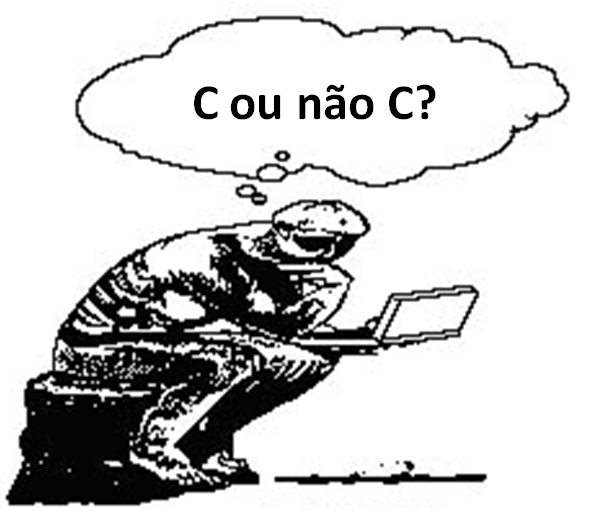
\includegraphics[width=7cm]{images/pensamento.png}
  		\end{center}
	\end{frame}
	
	\begin{frame}{Pensamento}
		\begin{columns}
			\column{.4\textwidth}  		
		  		\begin{center}
		    		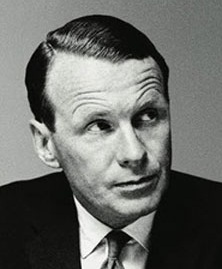
\includegraphics[height=.5\textheight]{images/ogilvy.jpg}
		  		\end{center}
			\column{.6\textwidth}  		
				\begin{block}{Frase}
					\begin{center}
						{\large As normas existem para \\a obediência dos tolos e \\ para a orientação dos sábios.}
					\end{center}
				\end{block}		  		
		  		\begin{block}{Quem?}
		  			\begin{center}
						{\bf David Ogilvy (1911-1999)} \\Publicitário inglês.
					\end{center}
				\end{block}
		\end{columns}
	\end{frame}   
    
    \section{Revisão}
	\begin{frame}{Conceitos}
		\begin{itemize}
			\item Digrafo \pause
			\item Arco \pause 
			\item Ponta (inicial e final)	\pause
			\item v-w (sair e entrar) \pause
			\item Vizinhança \pause
			\item Tamanho do digrafo: \pause V + A \pause
			\item Arcos paralelos e antiparalelos \pause
			\item Leque de saída e de entrada \pause
			\item Grau de saída e de entrada \pause
			\item Fonte, sorvedouro e vértice isolado \pause
			\item $A(G) \subset V(G)^2$ 
		\end{itemize}
	\end{frame}
	\begin{frame}{Conceitos}
		\begin{itemize}
			\item Digrafo completo \pause
			\item Torneio \pause
				\begin{itemize}
					\item em um torneio $\rightarrow$ $A = V(V-1)/2$ \pause
				\end{itemize}
			\item Digrafo denso \pause
			\item Digrafo esparso \pause
			\item Digrafo simétrico \pause = Grafo \pause
			\item Subdigrafo \pause
				\begin{itemize}
					\item Subdigrafo gerador \pause
					\item Subdigrafo induzido \pause
					\item Subdigrafo próprio \pause
					\item Subdigrafo induzido por $X$ \pause
				\end{itemize}
			\item Superdigrafo \pause
			\item Um subdigrafo de um grafo não é necessariamente um grafo
		\end{itemize}
	\end{frame}
	
	\begin{frame}{Conceitos}
		\begin{itemize}
			\item Representação dos vértices \pause
			\item Representação dos arcos \pause
				\begin{itemize}
					\item Matriz de adjacências \pause
					\item Lista de adjacências
				\end{itemize}
		\end{itemize}
	\end{frame}
	
	\section{Digrafos - Matriz de Adjacências}
	\begin{frame}{Representação com Matriz de Adjacências}
		\begin{block}{Estrutura básica}
			\begin{center}
	    		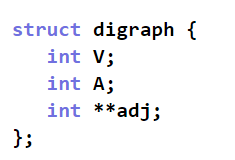
\includegraphics[height=.25\textheight]{images/digrafo.png}
	  		\end{center}
		\end{block} \pause
		\begin{block}{Digrafo}
			\begin{center}
	    		
\includegraphics[height=.1\textheight]{images/digrafo-ponteiro.png}
	  		\end{center}
		\end{block}
	\end{frame}
	
	\begin{frame}{Representação com Matriz de Adjacências}
		\begin{block}{Inicialização}
			\begin{center}
	    		\includegraphics[height=.3\textheight]{images/digraph-init.png}
	  		\end{center}
		\end{block}
	\end{frame}
	
	\begin{frame}{Representação com Matriz de Adjacências}
		\begin{block}{Inicialização da matriz}
			\begin{center}
	    		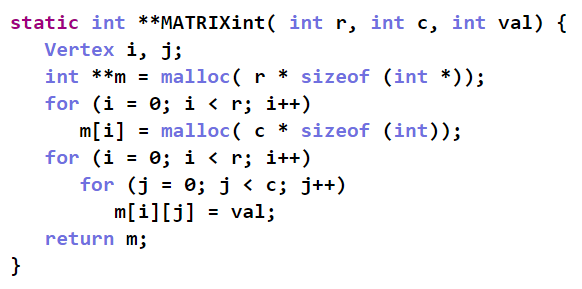
\includegraphics[height=.5\textheight]{images/matriz-adjacencias.png}
	  		\end{center}
		\end{block}
	\end{frame}
	
	\begin{frame}{Representação com Matriz de Adjacências}
		\begin{block}{Inserção}
			\begin{center}
	    		\includegraphics[height=.3\textheight]{images/digraph-insert-a.png}
	  		\end{center}
		\end{block} \pause
		\begin{block}{Remoção}
			\begin{center}
	    		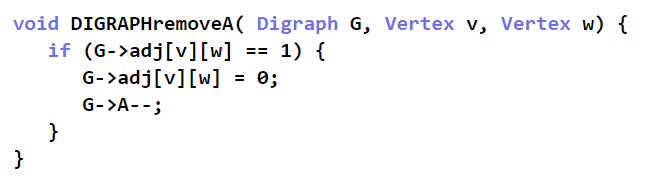
\includegraphics[height=.3\textheight]{images/digraph-remove-a.png}
	  		\end{center}
		\end{block}
	\end{frame}	
	
	\begin{frame}{Representação com Matriz de Adjacências}
		\begin{block}{Exibição}
			\begin{center}
	    		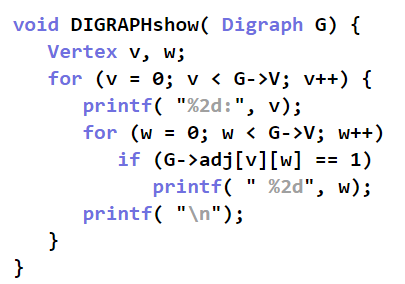
\includegraphics[height=.5\textheight]{images/digraph-show.png}
	  		\end{center}
		\end{block}
	\end{frame}
	
	\section{Digrafos - Lista de Adjacências}
	\begin{frame}{Representação com Lista de Adjacências}
		\begin{block}{Estrutura básica}
			\begin{center}
	    		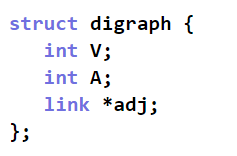
\includegraphics[height=.25\textheight]{images/lista/digraph.png}
	  		\end{center}
		\end{block} \pause
		\begin{block}{Digrafo}
			\begin{center}
	    		
\includegraphics[height=.1\textheight]{images/lista/digraph-ponteiro.png}
	  		\end{center}
		\end{block}
	\end{frame}
	
	\begin{frame}{Representação com Lista de Adjacências}
		\begin{block}{Nó e Ligação}
			\begin{center}
	    		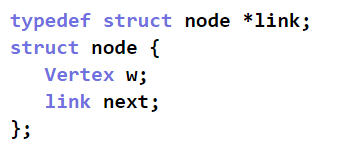
\includegraphics[height=.3\textheight]{images/lista/node.png}
	  		\end{center}
		\end{block} \pause
		\begin{block}{Novo nó}
			\begin{center}
	    		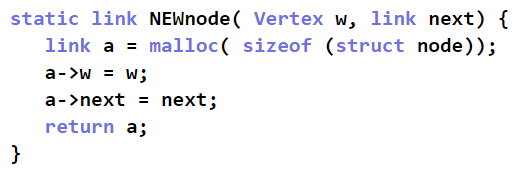
\includegraphics[height=.3\textheight]{images/lista/new-node.png}
	  		\end{center}
		\end{block}
	\end{frame}
	
	\begin{frame}{Representação com Lista de Adjacências}
		\begin{block}{Lista de adjacências}
			\begin{center}
	    		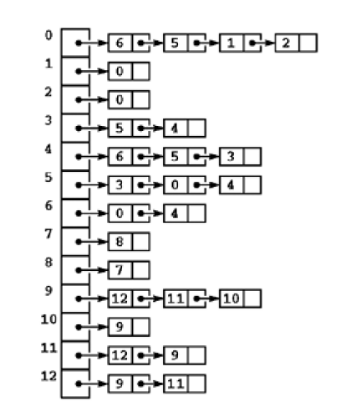
\includegraphics[height=.5\textheight]{images/lista/imagem.png}
	  		\end{center}
		\end{block}
	\end{frame}
	
	\begin{frame}{Representação com Lista de Adjacências}
		\begin{block}{Inicialização}
			\begin{center}
	    		\includegraphics[height=.6\textheight]{images/lista/digraph-init.png}
	  		\end{center}
		\end{block}
	\end{frame}	
	
	\begin{frame}{Representação com Lista de Adjacências}
		\begin{block}{Inserção}
			\begin{center}
	    		\includegraphics[height=.4\textheight]{images/lista/digraph-insert-a.png}
	  		\end{center}
		\end{block}
	\end{frame}
	
	\begin{frame}
		\titlepage
	\end{frame}
	
\end{document}